\documentclass{article}


\usepackage{authblk}
\usepackage{listings, chngcntr}
\usepackage{multicol}
\usepackage{textcomp}
\usepackage{float}
\usepackage[T1]{fontenc}
\usepackage{indentfirst}
\usepackage{graphicx}
\usepackage{array}
\usepackage{caption} 
\usepackage{hyperref}
\usepackage{verbatim}
\usepackage{float}
\usepackage{subcaption}
\usepackage{gensymb}
\usepackage{amsmath}
\usepackage{geometry}
\usepackage{multirow}
\usepackage{listings}


\geometry{
    a4paper,
    left=30mm,
    right=30mm,
    top=30mm,
    bottom=40mm
}

\begin{document}

\title{Electron Spin Resonance on Nitrogen-Vacancy center}
\author[1]{Woojin Han}
\affil[1]{Seoul National University, Seoul 151-747, Korea}
\maketitle

\begin{abstract}
    The experiment aimed to find electron spin resonance (ESR) in well-prepared settings, but this goal was not achievable due to insufficient lab settings.
    Therefore, this report elaborates on the detailed mechanisms of ESR of the Nitrogen-Vacancy Center (NV center).
    The limitations of the current setup are highlighted by estimating the noise and providing improvements for future settings.
    Prior research on the NV center's basic electric structures and energy gaps is revisited.
    The relationship between the magnetic field and spin states, as explained by the Rabi model, and the theoretical background of ESR is well understood.
    The experimental setups are described in detail, with a schematic plot of the setting.
    The ESR results across various frequencies and amplitudes are depicted.
    On the challenges faced, the findings and recommendations will be applied in a few months to have physical results.
\end{abstract}

\section{Introduction}
The original purpose of this report and the experiment was to find electron spin resonance(ESR) in well-prepared settings, but the goal is not achievable due to insufficient lab settings.
Therefore in this report, I elaborate on the detailed mechanisms of the ESR of the Nitrogen-Vacancy Center(NV center) in mathematical models and the apparatus we have in the lab.
Moreover, the limitation we have shall be revealed by the appropriate noise estimation so that the report may help the settings work well.
In the rest of the subsection in the Introduction, the prior researches are revisited.
The basic electric structures of the NV center and its energy gap are studied.
The relation between the magnetic field and the spin states, in the Rabi model is visited, and the calculational backgrounds of ESR are fully understood.
In \ref{section: experiment}, the experimental setups are explained.
The manual of each apparatus and the setting are schematically plotted.
The ESR result in varies of frequency and the amplitude is given, and the improvements of the settings are also provided at \ref{section: improvements}


\subsection{Theory: NV Center}
\label{section: theory}
The Nitrogen-Vacancy center (NV center) is the crystal structure that has a nitrogen atom that is adjacent to a vacancy in the diamond lattice.
The negatively charged NV center has diverse research on its electric and optical structures.
The leading theory on its electric structure, six electron models in the molecular orbital suggested in \cite{sixelectron} is considered correct until now.
The energy distribution of each state is calculated from scratch, for example, DFT-LSDA or \textit{Ab inittio}.
The theory assumes the energy state could be obtained from the linear combinations of the atomic orbital nearby, which is empirically validated by Hartree–Fock methods.
Also, the well-defined total spin and angular momentum eigenstates of the multi-electron problems are suggested, which can be validated by many experiments.
Fig. \ref{fig: six electron energy states} shows the possible energy states constructed from dangling $sp^3$ orbitals from the carbon atom and the nitrogen atom, which have a total number of $3\times1 + 2 + 1 = 6$ electrons.
Three electrons are obtained from single electrons of carbon, nitrogen donates two electrons to the vacuum, and the negatively charged electron is located in the relative energy sink, vacancy.
The other electron possesses the stable molecular orbital, while two electrons in LUMO build complex spin states to make NV$^-$ center have its unique optical properties.
The parent crystal structure, diamond, has $C_{3\nu}$ symmetry.
Therefore, the spin wave functions of the NV center could be theoretically calculated.
The triplet state has the ground state of $ ^3A_2$, where $3$ denotes its total spin $2\times1+1$, and the character $A$ denotes the nondegenerate state.
The excited triplet state is $ ^3E$, and $E$ denotes a degeneracy of 3.
There are also a singlet state, $ ^1E$ and $ ^1A_1$.
The relative energy plot is depicted in Fig. \ref{fig: electronic structure}.
Each radiative transition has a bold arrow, whereas nonradiative transitions have dotted lines.
Each triplet state has a total spin of $S = 1$, therefore having $m_s = 0, \pm 1$ fine structure each.
For zero field situations, the energy of that $ m_s$ should be degenerate.
However, the spin-orbital coupling induces energy splits between different $m_s$, which is called zero-field splitting(ZFS).
The ZFS energy gap of the ground state is $2.88 GHz$ reported (\cite{nv}).
The exact mechanisms from triplets to singlet transitions are not known, but the phononic action is expected (\cite{nvphonon}).
Experimentally, the mechanical strain changes the transition proportion to the singlet state, the phononic contribution is a rational guess so far.

\begin{figure}[ht]
    \centering
    \begin{subfigure}[b]{5cm}
        \centering
        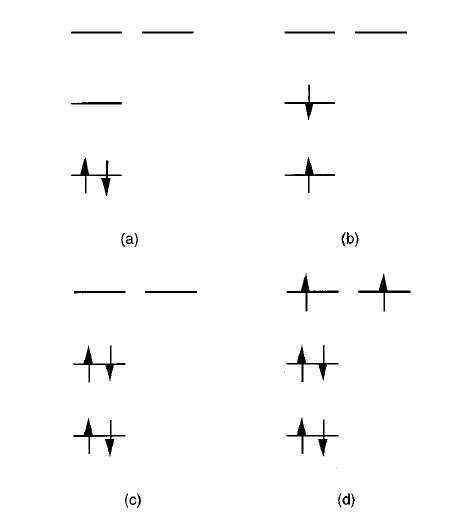
\includegraphics[width=5cm]{./figs/six_electron_model.png}
    \end{subfigure}
    \hfill
    \caption{
        The molecular orbital configuration for multiple numbers of electrons (\cite{sixelectron}).
        (a) for $n = 2$ ground state (b) for $n = 2$ excited state (c) for $n = 4$ (d) for $n = 6$
    }
    \label{fig: six electron energy states}
\end{figure}
\begin{figure}[ht]
    \centering
    \begin{subfigure}[b]{7cm}
        \centering
        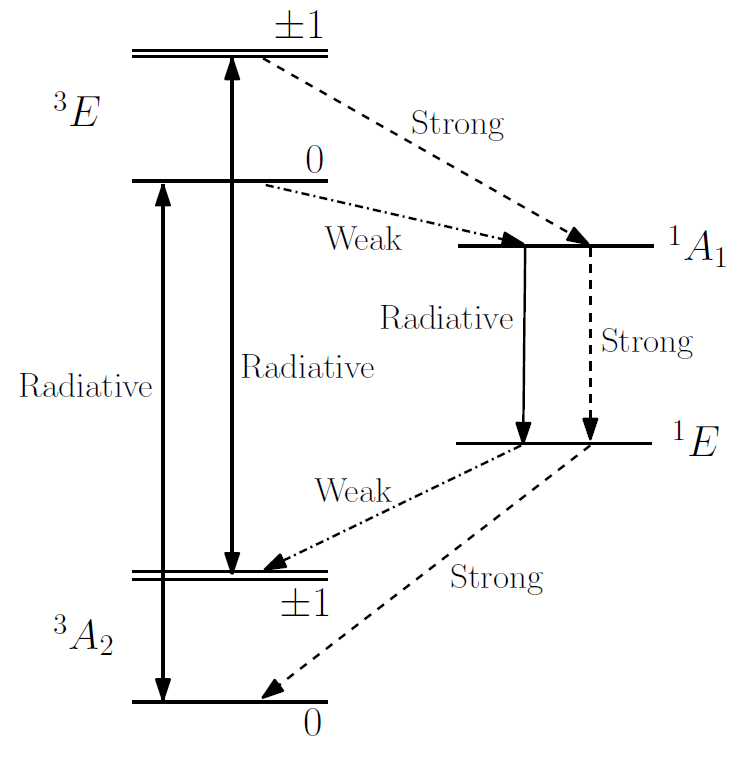
\includegraphics[width=7cm]{./figs/electronic structure.png}
    \end{subfigure}
    \hfill
    \caption{
        The relative energy plot of the electronic structure of NV$ ^-$ center is depicted in (\cite{nv}).
        $ ^3A_2$ and $ ^3E$ are both triplet state, have $m_s = 0, \pm 1$ fine structures.
        The radiative interaction among those states is well calculated, and its energy gap is also given.
        $ ^1A_1$ and $ ^1E$ are both singlet states and have nonradiative interaction with triplet states.
        The exact mechanisms of mediating energy, that change its total spin are not conserved and have no certain consensus.
    }
    \label{fig: electronic structure}
\end{figure}

\subsection{ESR}
Both $m_s = 0, \pm 1$ states are luminescence from green light (typically $532nm$) and emmit $637nm$ spectra red light.
The singlet state also has radiative transition, but its radiation spectrum is at the infrared region $1042nm$.
The excited triplet state $ ^3E$ has non-radiative phononic relaxation to the singlet state.
$m_s = \pm 1$ spin states are more likely to enhance the transition rate to singlet state, due to its orbital configuration. (\cite{preference})
Therefore, the luminescence intensity of the $m_s = 0$ $ ^3A_2$ states is larger than the $m_s = \pm 1$ states, the optically detected magnetic resonance(ODMR) is possible.
The magnetic field applied to the crystal may change the inter-state spin conditions.
The ZFS energy gap is around the microwave region and has resonant properties.
If the lower energy wave is emitted, the electrons are not able to excite to the higher state.
If the higher energy wave is emitted, the angular momentum of the total system cannot be conserved when the light is absorbed.
By the homogeneous phonon broadening and the temperature effects, the resonance valley forms the negative Lorentzian-like peak.
It is experimentally supported due to the line width drops significantly compared to the one at room temperature near $5K$ reported (\cite{lowtemp}).
Without the magnetic field applied, the $m_s = \pm 1$ state does not split, therefore there is one resonance peak near $2.88GHz$.
The mechanisms of spin changing by microwave is presented at \ref{section: Rabi}.

\subsection{Rabi rotation}
\label{section: Rabi}
When the quantum spin state experiences the magnetic field, the Hamiltonian is given as follows.
$\hat{\vec{S}}$ is the respective well-defined spin operator, $g$ is gyromagnetic ratio, and $\mu_B$ is the Bohr magnetic momment.
For the NV$ ^-$ center, the triplet state is assumed to have a proper total spin operator, and the Rabi rotation can be considered.
\begin{equation}
    \hat{H} = g\mu_B \vec{B} \cdot \hat{S}
\end{equation}
The microwave applied to the system takes the role of AC magnetic field.
Since its magnetic field magnitude is not bigger than the other external magnetic field, the perturbational Hamiltonian is valid.

\begin{equation}
    \hat{H} = g\mu_B \left( B_z \hat{S_z} + B_x \cos(\omega t) \hat{S_x} \right)
\end{equation}

The high-frequency approximation, in each of the perturbed $\omega \gg E/\hbar$, the Hamiltonian can be roughly solved by rotating wave approximation(RWA).
For the Rabi frequency $\Omega_R = g\mu_B B_1$, the probability density dynamics of each spin state are given as follows.

\begin{equation}
    P_{0\rightarrow1} (t) = \sin^2\left(\frac{\Omega_R t}{2}\right)
\end{equation}

This means by the time exposed to the microwave, the probability density fluctuates to be at $m_s = 0$ or shifted to $m_s = \pm1$ states.
Since ESR detects the ratio of the probability density of each spin state, the exposed time is proportional to the intensity results.
Moreover, the intensity of the microwave is correlated to the square of the magnetic field affecting the crystal, which is linear to the Rabi frequency.
So, with the appropriate experiment setting, by changing the intensity or exposure time of the microwave at the resonance frequency, the ESR peak value should fluctuate by the Rabi model prediction.
However, the reported experimental Rabi figures seem to converge to a certain value, not fluctuating between $m_s = 0, \pm 1$ states.
That is the effect of perturbations, in which the fringe Hamiltonian affects phase shifts to the spin states, to vaguely spread out to the degenerate spin states.
Therefore, the experimental aim should be searching for the first fluctuation point, fully exiting the ground spin state to $m_s = \pm 1$.

\section{Experiment}
\label{section: experiment}
The experiment was performed using the gated photon counter, the signal generator, and the pulse blaster placed in Seoul National University 26-418.
The gated photon counter is model SR400 and its performance is denoted at (\cite{photoncounter}).
The signal generator is model MG3700A and its performance is written at (\cite{signalgenerator}).
The function generator is model AFG3000C and its performance is depicted at (\cite{functiongenerator}).
Lastly, the pulse blaster is made by spin core, and its manual can be found at (\cite{pulseblaster}).
The experiment was done four times in 2024 June and its noticeable differences are all denoted below.

\begin{figure}[ht]
    \centering
    \begin{subfigure}[b]{7cm}
        \centering
        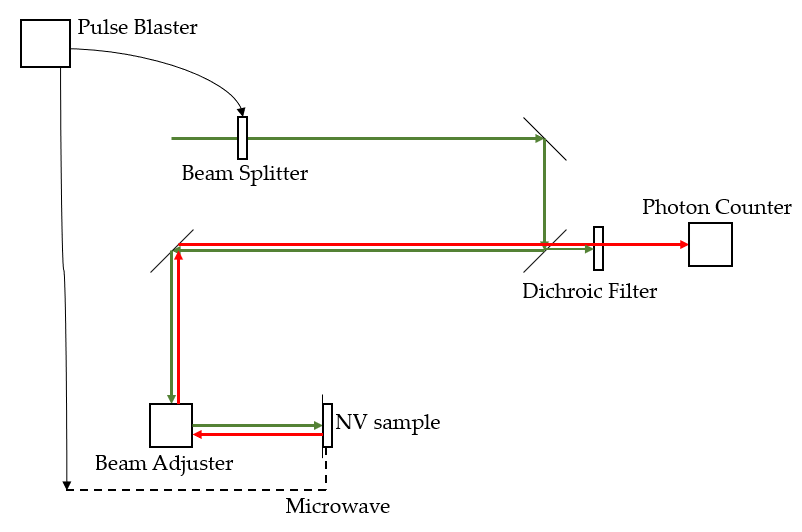
\includegraphics[width=7cm]{./figs/apparatus.png}
    \end{subfigure}
    \hfill
    \caption{
        The schematic picture of the apparatus.
        The green arrow is the green laser of wavelength 532 $nm$, expected to make the NV sample emit red light.
        The emitted red light follows the track of mirrors and passes through the dichroic filter.
        Finally, the photon counter counts the red light signal in pre-scheduled gate width.
        All of those processes are managed by the pulse blaster.
    }
    \label{fig: apparatus}
\end{figure}

The pulse blaster processes the microwave and the photon counters gate times in repeating timescales.
They run in $120\mu s$ for each loop, and the microwave is emitted for $30 ns$ each.
After the microwave emission, the photon counter gates open.
The counted photons are interpreted as the EPS intensity.
To make the value in units, the photon counter gate opens after $59.7 \mu s$.
The base counted photons are considered as the spin 0 state signal.
Each data point is calculated from 100 reciprocal experiments.
Finally, the EPS signal is induced from their ratio.
The experimented result is depicted in Fig \ref{fig: result}.
In the non-resonant state, the ESR signal has a respective value of 1 which means the magnetic field of the microwave is not enough to excite the electrons.
It has a negative peak at $2.87GHz$, where the resonant frequency possesses, has a signal value of $0.95$.
The plot seems elegant and the ESR might seem successfully done, but the peak height is too small that we can not claim the resonance property.
Therefore, the experiment is not successful enough but has half of its aim done.

\begin{figure}[ht]
    \centering
    \begin{subfigure}[b]{7cm}
        \centering
        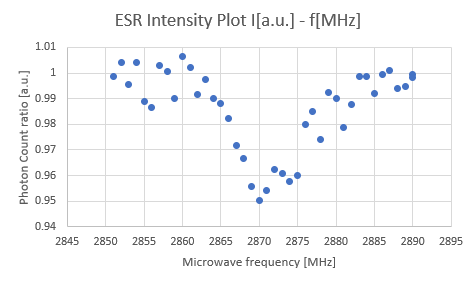
\includegraphics[width=7cm]{./figs/result.png}
    \end{subfigure}
    \hfill
    \caption{
        Plot of the EPS signal by changing microwave frequency.
        The peak position is $2.87 GHz$, which is predicted in the previous reports.
    }
    \label{fig: result}
\end{figure}


\subsection{Possible improvements}
\label{section: improvements}
From the result of the experiment, three things could be guessed.
The experimental setup might have fatal flaws in that the result is fully contaminated by errors, and it was pure luck to have a peak at the resonance point.
However the peak position and its peak width seem clear, so it is more valid to think that was not a full random error controlling the plot, but a weak signal can be caught by our system.
With the assumption, our microwave setup could be at an exact Rabi intensity that the phase might shift at the angle of $2 \pi$.
But the second guess returns to nothing with Fig \ref{fig: result2}.
The figure is the EPS signal with microwave intensity, and the signal is random.

\begin{figure}[ht]
    \centering
    \begin{subfigure}[b]{7cm}
        \centering
        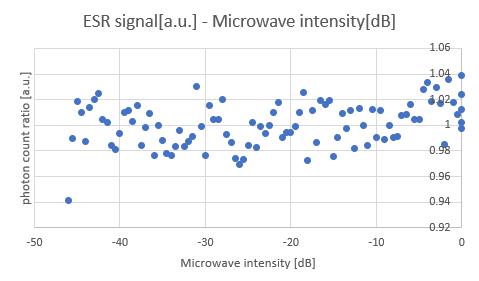
\includegraphics[width=7cm]{./figs/result2.png}
    \end{subfigure}
    \hfill
    \caption{
        Plot of the EPS signal by changing microwave Intensity.
        Seems no signal is been found
    }
    \label{fig: result2}
\end{figure}
The last guess, and the only possible guess is that the system has a lot of white noises.
Not like the green laser, the microwave has a chance not to emit on all of the NV centers properly.
Therefore, some proportion of the NV center experiences the Rabi rotation, while the other NV center just gets the green light and emits the red light back.
It makes a white signal at the back of each photon gate counter and reduces the EPS signal size.
This guess seems valid since the microwave is not applied on the surface of the sample but by the legacy platform.
I was not able to look into the sample legacy until today, but after this report, the first task to fix the NV center is to look at how the microwave affects the sample.

\section{Conclusion}
In this report, the theory of the NV center and the EPS is deeply studied.
The six-electron model of the molecular orbital is visited.
The symmetry of the triplet state and the singlet states are fully known from prior research.
The ODMR and EPS actions of microwaves and their resonance nature are now understood.
Also, the current apparatus and the experiment results are plotted and analyzed.
With a deep analysis of the result, the flaws of the setup might be revealed.
Moreover, the program time synchronization problem also remains.
For the higher freedom to this modification, code refactoring is unavoidable.



\bibliography{esr_ref}
\bibliographystyle{plain}
\end{document}
